% !TeX TS-program = pdflatex
% !TeX encoding = UTF-8
% !TeX spellcheck = en_GB
% !TeX root = contest-main.tex
\documentclass[]{beamer}

\usepackage[T1]{fontenc}
\usepackage{textcomp}
\usepackage[utf8]{inputenc}
\usepackage{babel}
%\geometry{}

\graphicspath{{../r/plots/}}

\usepackage{booktabs}
%\usepackage{caption}
%\captionsetup{format=hang,labelsep=colon}%,font={small,rm},labelfont={sf,bf}}
%\captionsetup[table]{skip=-0.9\medskipamount,position=top}

\usepackage[ruled,linesnumbered]{algorithm2e}
\SetNlSty{texttt}{}{}
\SetKw{Or}{or}
\SetKw{And}{and}
\SetKw{Not}{not}

% -------- %
\title{Presentation title}
\subtitle{Presentation subtitle}
\author{Name Surname \and Name Surname \and Name Surname}
\institute[UniFi]{MSc in AI, University of Florence}
\date{May 21, 2024}
%\logo{\includegraphics[width=0.2\textwidth]{./Figures/logo}}
%\titlegraphic{\includegraphics{./Figures/logo}}
% -------- %

\usepackage{appendixnumberbeamer}
%\mode<presentation>
\usetheme[progressbar=foot,numbering=counter]{metropolis}
%\useoutertheme[right]{sidebar}
\setbeamercovered{dynamic}
%\setbeamertemplate{blocks}[default]%[shadow=true]
\setbeamertemplate{sections/subsections in toc}[circle]
\setbeamertemplate{items}[circle]
\setbeamertemplate{navigation symbols}{}
\metroset{block=fill}

%\mode<all>

% definizione degli enunciati matematici
%\theoremstyle{definition}
%\newtheorem{defs}{Definition}
%\theoremstyle{plain}
%\newtheorem{thm}{Theorem}

\usepackage{mathtools}
\newcommand{\numberset}{\mathbb}
\newcommand{\R}{\numberset{R}}
\DeclareMathOperator{\sign}{sign}
\DeclareMathOperator*{\argmin}{arg\,min}
\DeclarePairedDelimiter{\abs}{\lvert}{\rvert}
\DeclarePairedDelimiter{\norma}{\lVert}{\rVert}
\DeclarePairedDelimiter{\set}{\{}{\}}
\renewcommand{\epsilon}{\varepsilon}

\usepackage{siunitx}
\sisetup{%
	output-decimal-marker={.},group-separator={\,},%
	%	round-mode=places,round-precision=6,%
	table-parse-only,table-number-alignment=center%
}

%\usepackage{enumitem}

\usepackage{pgfplots} % + tikz
\pgfplotsset{compat=newest}
\usetikzlibrary{shapes,calc}

\tikzstyle{cloud} = [draw,ellipse,centered,text width=3.5em,text centered,
					inner sep=0.5pt,outer sep=0pt,fill=mLightBrown!20,font=\footnotesize]

\newcommand{\maxlike}{{\tiny ML}}

%\usepackage{pgfpages}
%\pgfpagesuselayout{4 on 1}[a4paper,border shrink=5mm,landscape]
%\usepackage{showframe}
\begin{document}

\pdfbookmark[1]{Title page}{cover}
\maketitle

% ------------------------------- %

\begin{frame}{Logistic Regression package}

\begin{columns}[T]
\begin{column}{0.5\textwidth}
TODO -- Formact code

\texttt{alpha = 1   \# Lasso = 1 -- Ridge = 0 -- 0 < Elastic < 1}
\texttt{cv.model = cv.glmnet(x.train, y.train, family = 'binomial', alpha = alpha)}
\texttt{best.lambda <- cv.model\$lambda.min}
\end{column}
\begin{column}{0.5\textwidth}
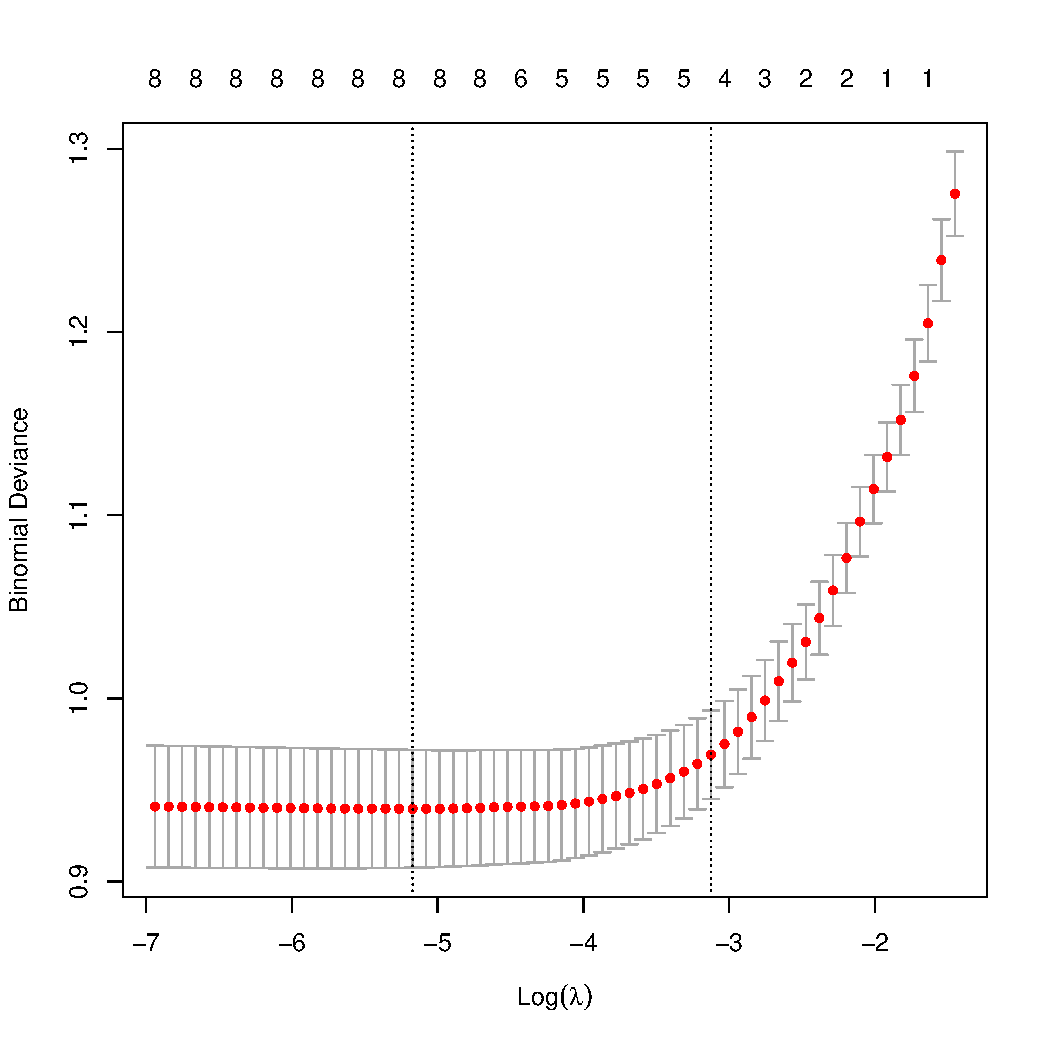
\includegraphics[width=0.85\columnwidth]{./Figures/logist/cv_lambda.pdf}
\end{column}
\end{columns}

\end{frame}

\begin{frame}{Ridge and Lasso variable importance}

\vspace*{-1em}\begin{columns}[T]
\begin{column}{0.5\textwidth}
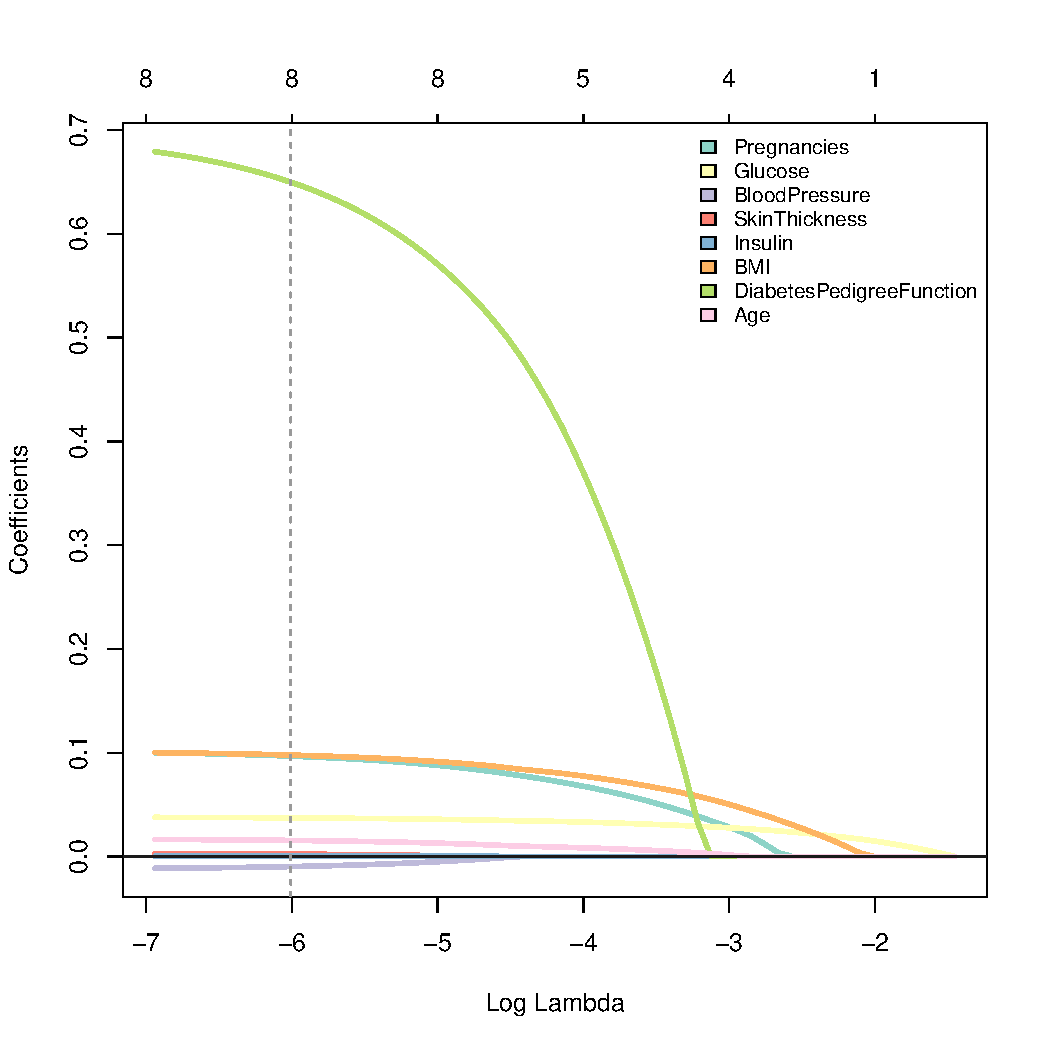
\includegraphics[width=0.85\columnwidth]{./Figures/logist/diabetes_lasso.pdf}
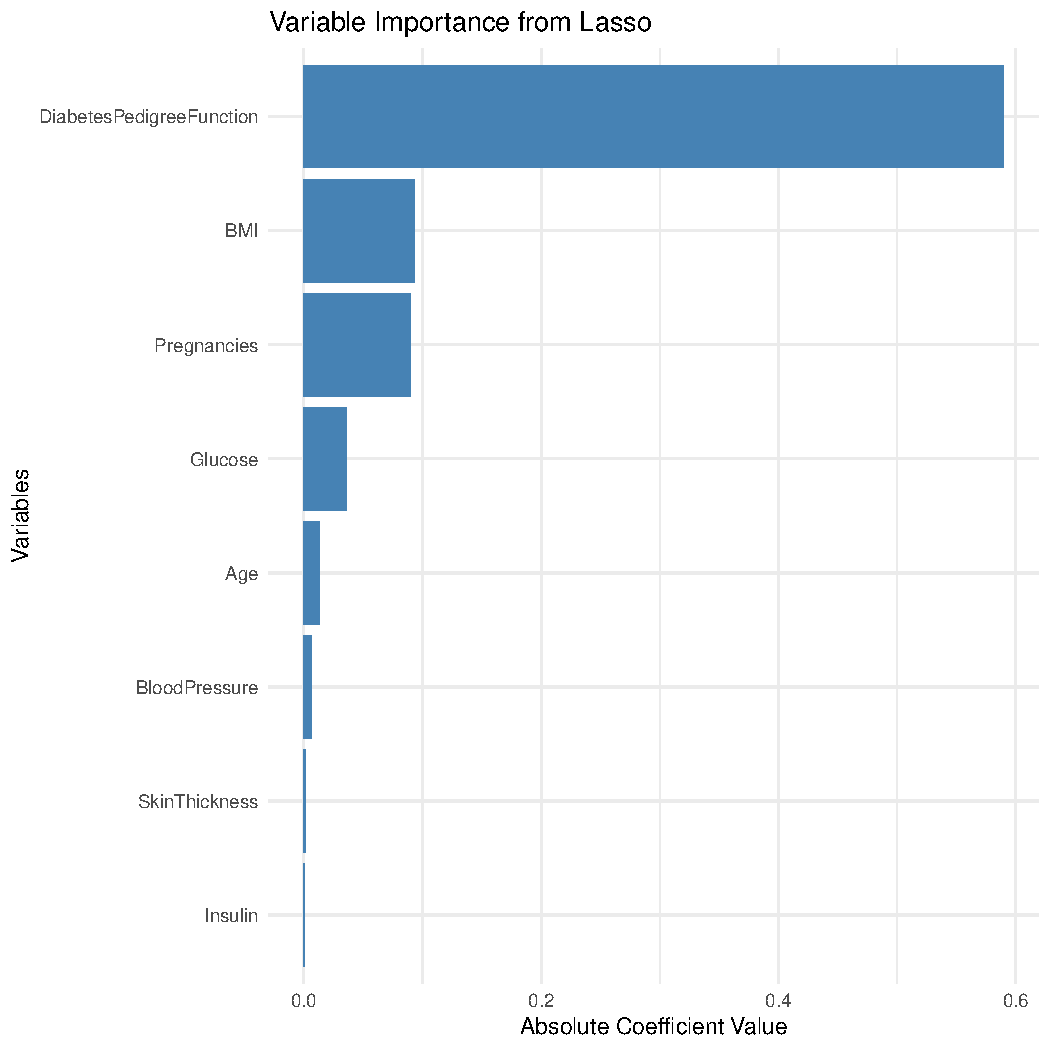
\includegraphics[width=0.7\columnwidth]{./Figures/logist/variable_importance_lasso.pdf}
\end{column}
\begin{column}{0.5\textwidth}
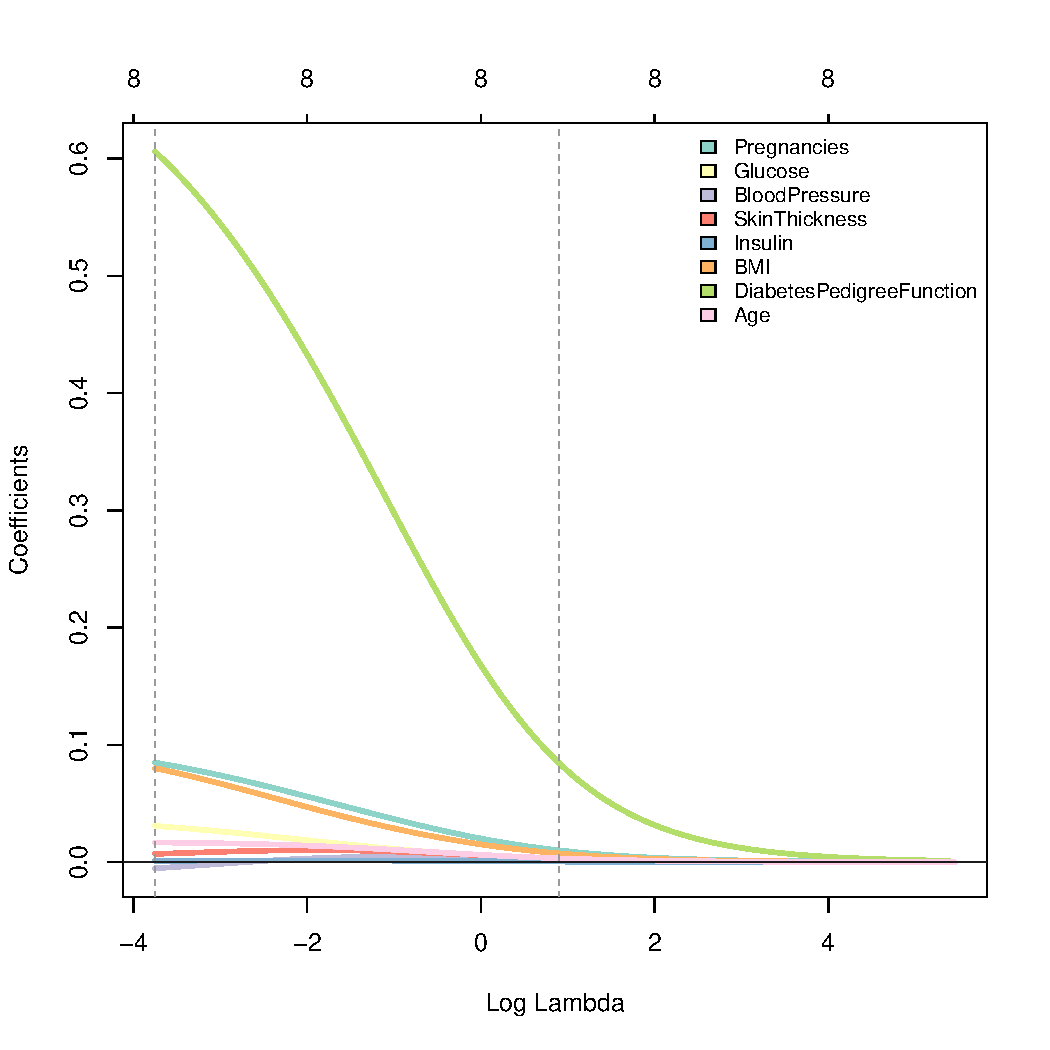
\includegraphics[width=0.85\columnwidth]{./Figures/logist/diabetes_ridge.pdf}
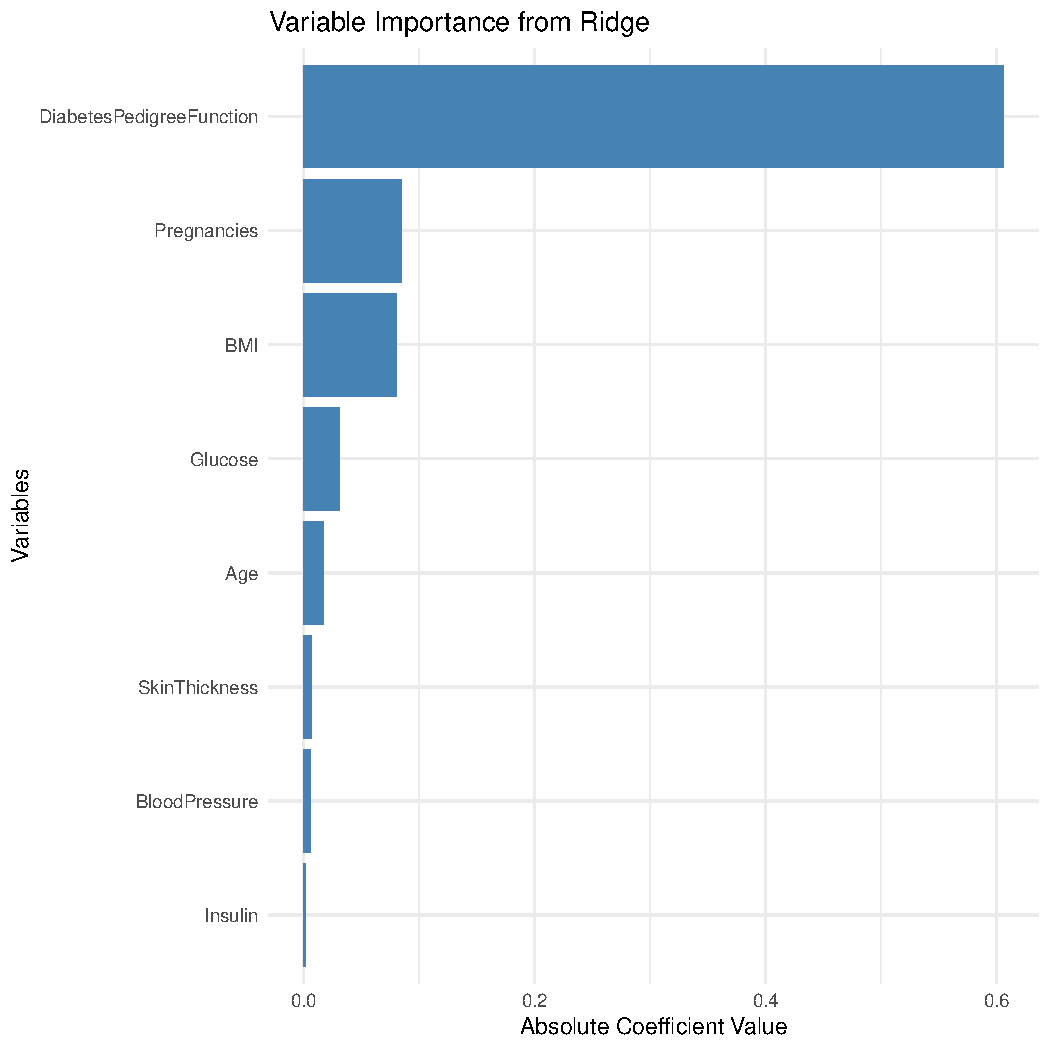
\includegraphics[width=0.7\columnwidth]{./Figures/logist/variable_importance_ridge.pdf}
\end{column}
\end{columns}

\end{frame}

\begin{frame}{ElasticNet and AdaLasso variable importance}

\vspace*{-1em}\begin{columns}[T]
\begin{column}{0.5\textwidth}
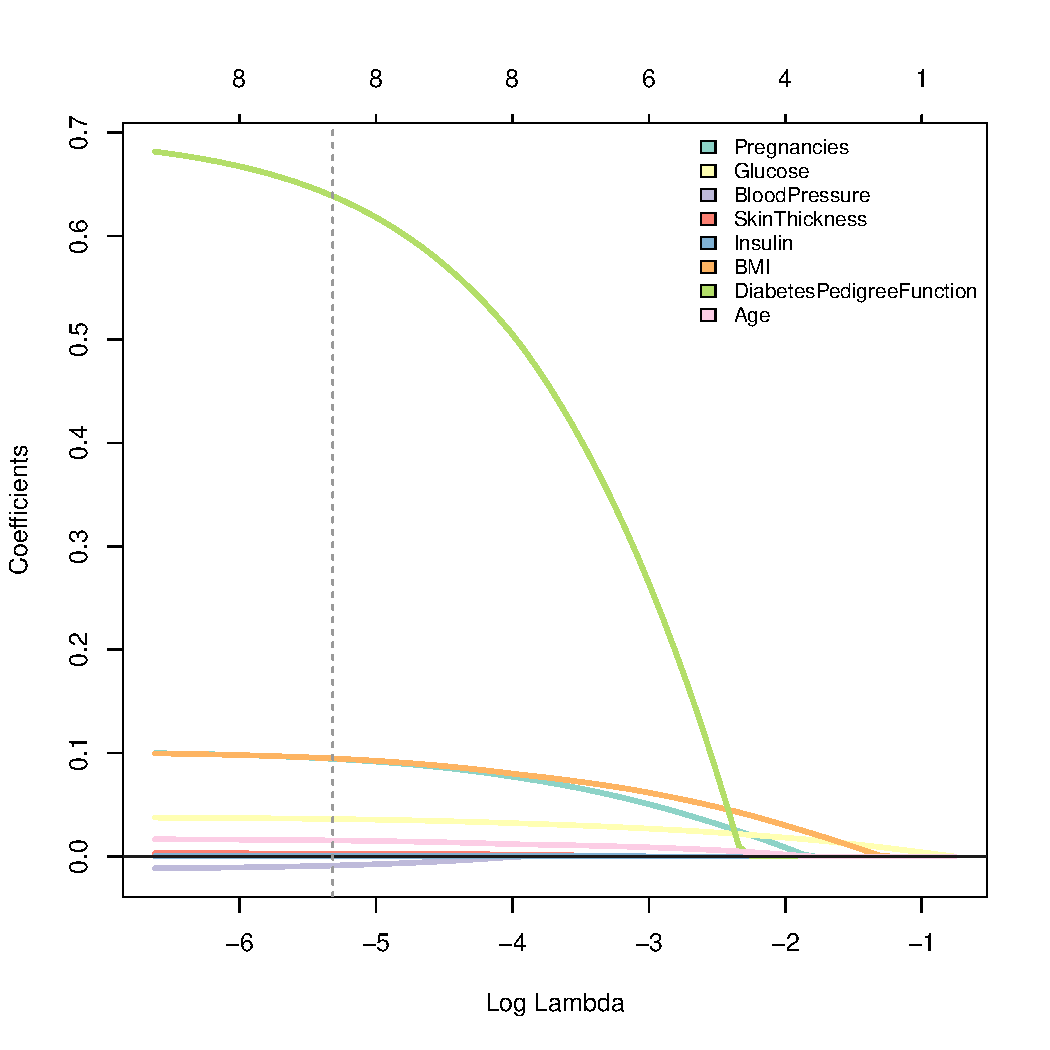
\includegraphics[width=0.85\columnwidth]{./Figures/logist/diabetes_elasticnet.pdf}
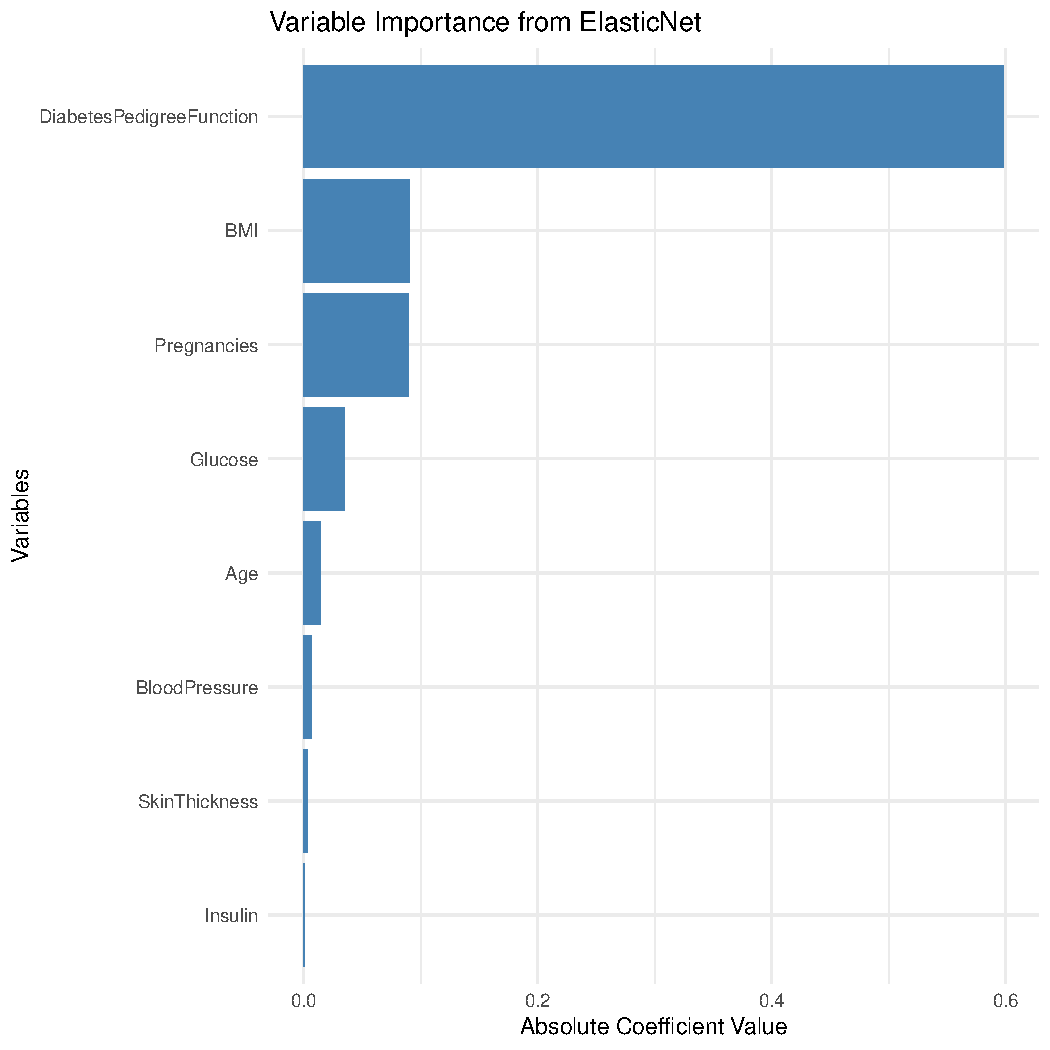
\includegraphics[width=0.7\columnwidth]{./Figures/logist/variable_importance_elasticnet.pdf}
\end{column}
\begin{column}{0.5\textwidth}
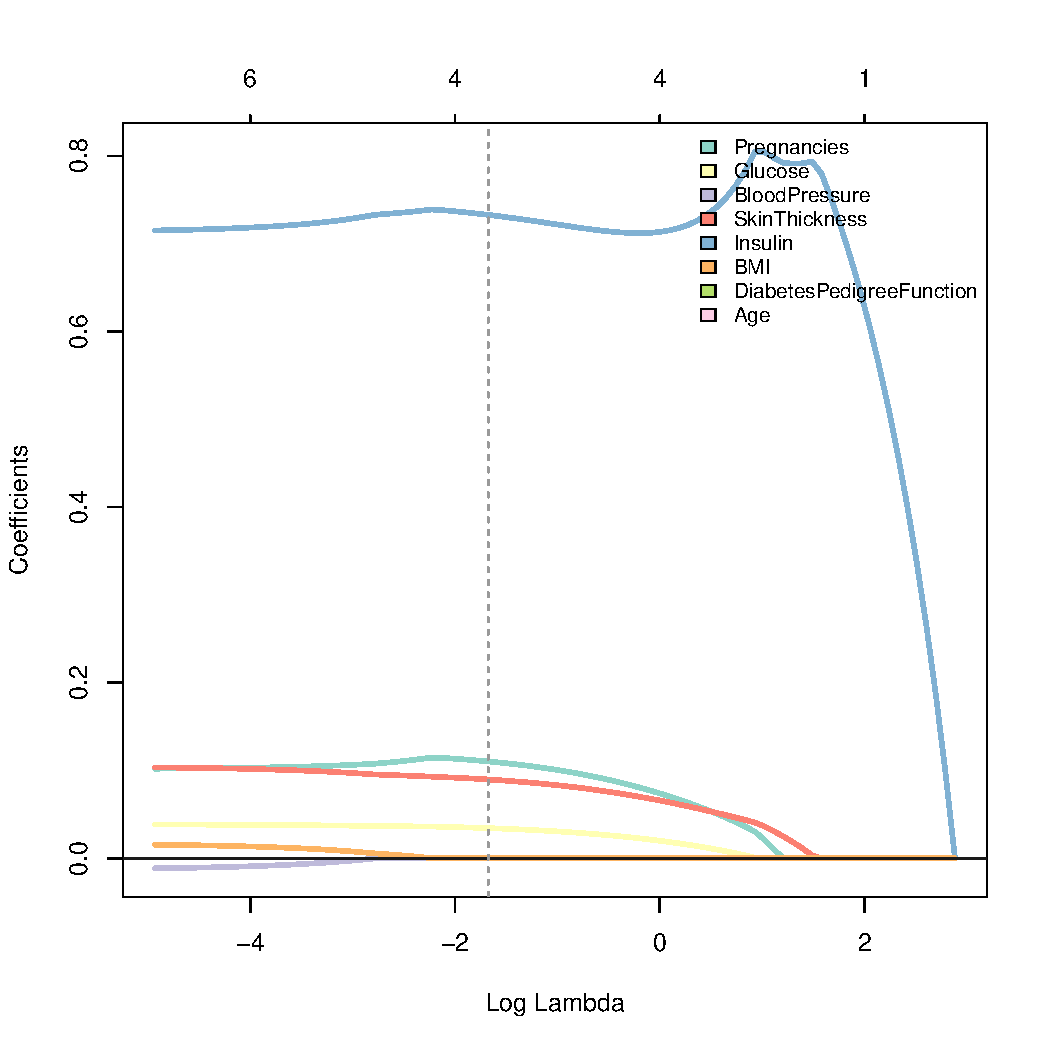
\includegraphics[width=0.85\columnwidth]{./Figures/logist/diabetes_adalasso.pdf}
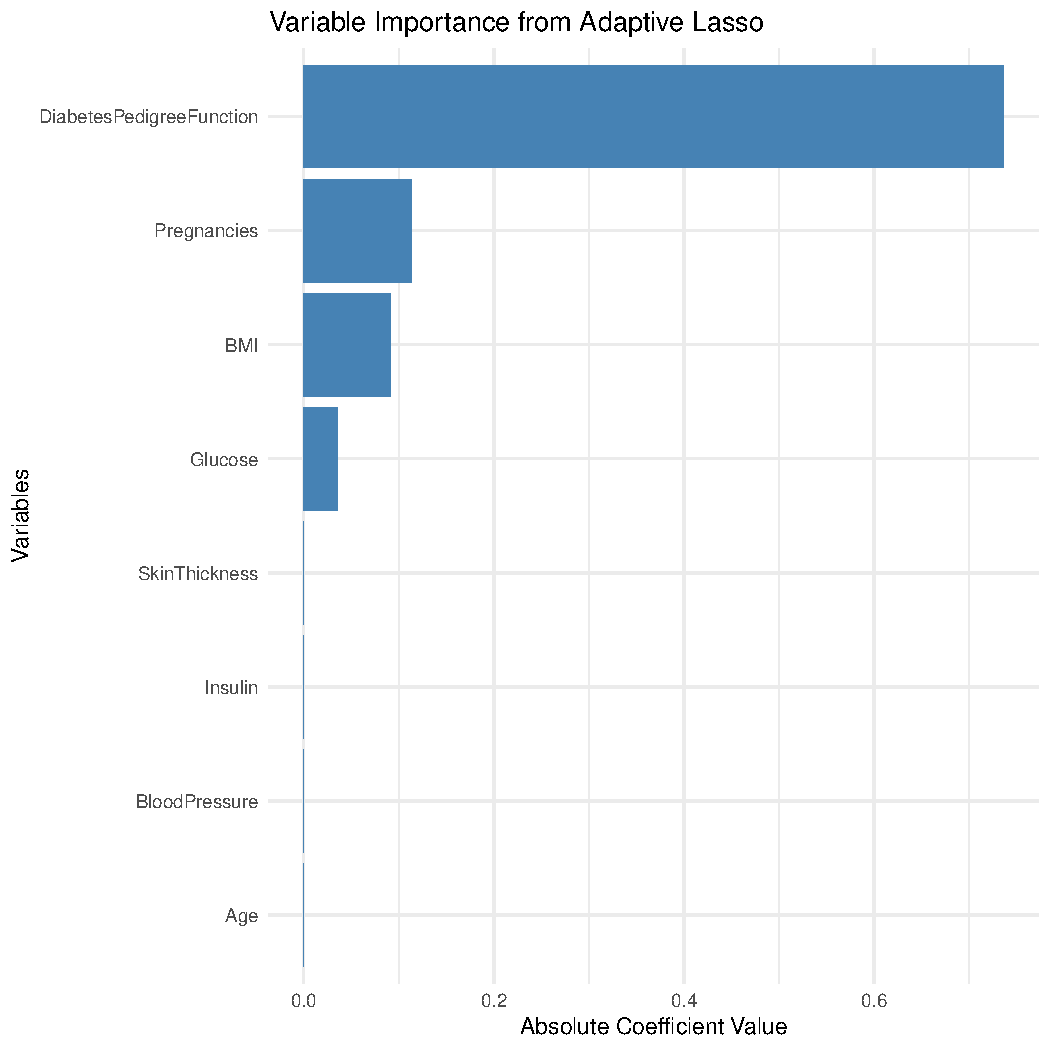
\includegraphics[width=0.7\columnwidth]{./Figures/logist/variable_importance_adalasso.pdf}
\end{column}
\end{columns}

\end{frame}

\begin{frame}{Results}
    \begin{table}
\sisetup{round-mode=places}
\resizebox{\textwidth}{!}{
\begin{tabular}{lS[round-precision=4]S[round-precision=4]S[round-precision=4]}
	Model & {Train score} & {Test score} & {\(\lambda\)} \\
	\midrule
	Lasso & 0.7714844 & 0.7695312 & 0.005678404 \\
	Ridge & 0.7695312 & 0.765625 & 0.02346324  \\
    ElasticNet & 0.7734375 & 0.7695312 & 0.008591009  \\
    AdaLasso & 0.7714844 & 0.7695312 & 0.005678404 \\
	\bottomrule
\end{tabular}}
\end{table}
\end{frame}
% !TeX spellcheck = en_GB

% ------------------------------- %
%% Random Forest Classifier %%
% ------------------------------- %

\begin{frame}{Random Forest for Classification}

{\small Package \texttt{\{randomForest\}}\vspace{-1.5ex}
\begin{itemize}\setlength{\itemsep}{-0.5ex}
	\item \lstinline|randomForest(formula, data=NULL, ntree=500, mtry=sqrt(p), importance=TRUE,|\texttt{\dots)}
	\item \lstinline|importance(x, type=NULL, class=NULL,|\texttt{\dots)}
    \item \lstinline|varImpPlot(x, sort=TRUE,|\texttt{\dots)}
    \item \texttt{x\$confusion}
    \item \texttt{x\$err.rate}
\end{itemize}}

{\texttt{x}} is a {\texttt{randomForest}} object;

{\texttt{ntree}} = number of trees grown;

{\texttt{p}} = number of predictors;

{\texttt{mtry}} = number of predictors sampled for splitting at each node.

\end{frame}

% ------------------------------- %

\begin{frame}{OOB Error}
\begin{columns}
\begin{column}{0.35\textwidth}

{\footnotesize \begin{itemize}
	\item $p$ = 8
	\item \texttt{mtry} = $\sqrt{p} \simeq 3$
	\item \texttt{ntree} = 500
	\item OOB estimate error rate: $24.41\%$
\end{itemize}}

\vspace{0.5cm}

\; Model selection:
{\footnotesize \begin{itemize}
	\item \texttt{ntree} = 111
	\item min OOB error rate = 0.2343
\end{itemize}}

\end{column}
\begin{column}{0.75\textwidth}
\begin{figure}
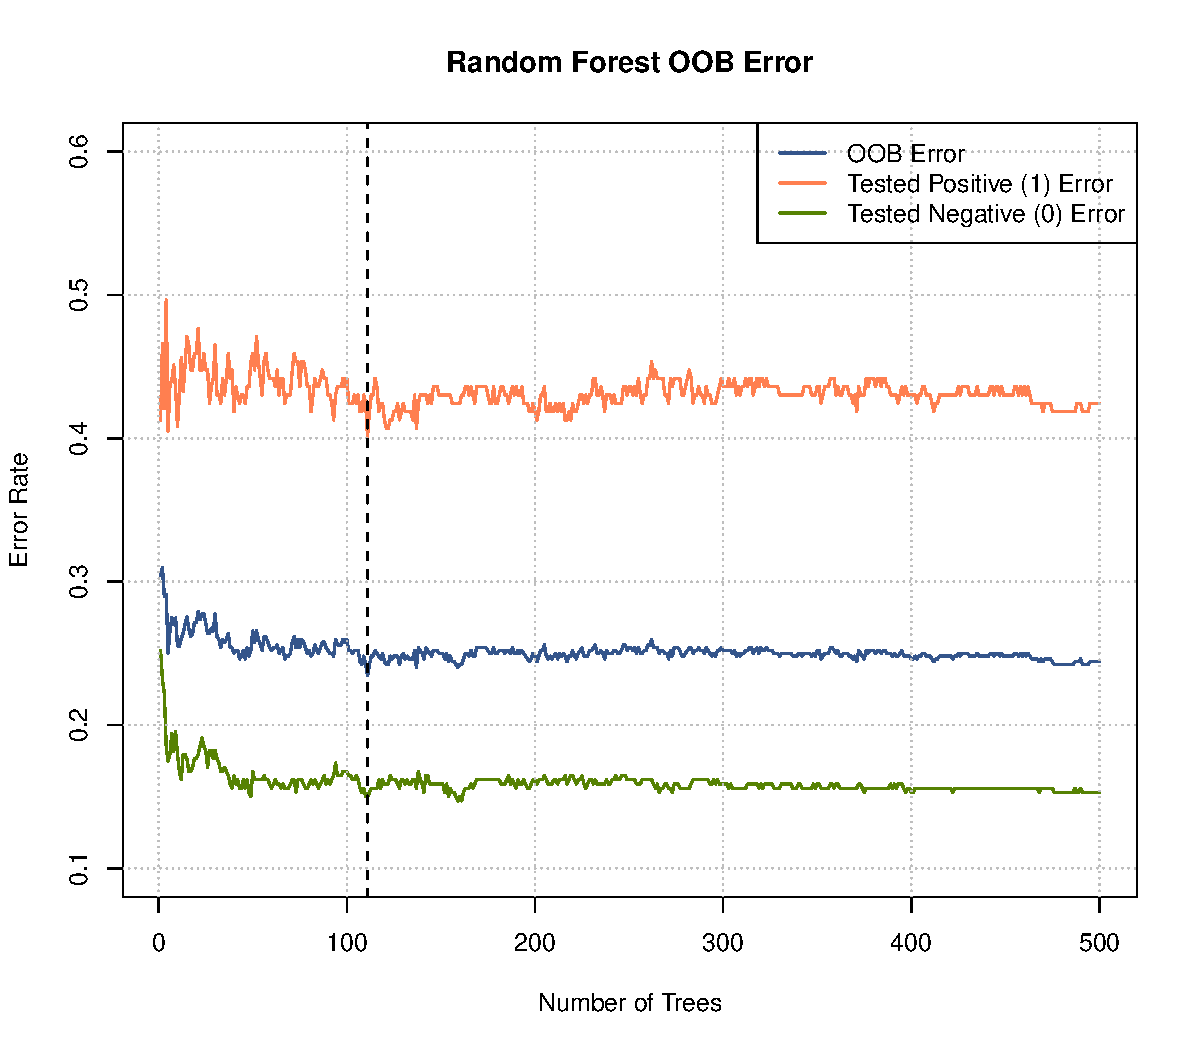
\includegraphics[width=1.05\columnwidth]{./Figures/forest/diabete_forest_error3.pdf}
\end{figure}
\end{column}
\end{columns}
\end{frame}

% ------------------------------- %

\begin{frame}{OOB Error}

\begin{columns}
\begin{column}{0.35\textwidth}
{\footnotesize \begin{itemize}
	\item $p$ = 8
	\item \texttt{mtry} = 4 
	\item \texttt{ntree} = 500
	\item OOB estimate error rate: $25\%$
\end{itemize}}

\vspace{0.5cm}

\; Model selection:
{\footnotesize \begin{itemize}
	\item \texttt{ntree} = 136
	\item min OOB error rate = 0.2226
\end{itemize}}

\end{column}
\begin{column}{0.75\textwidth}
\begin{figure}
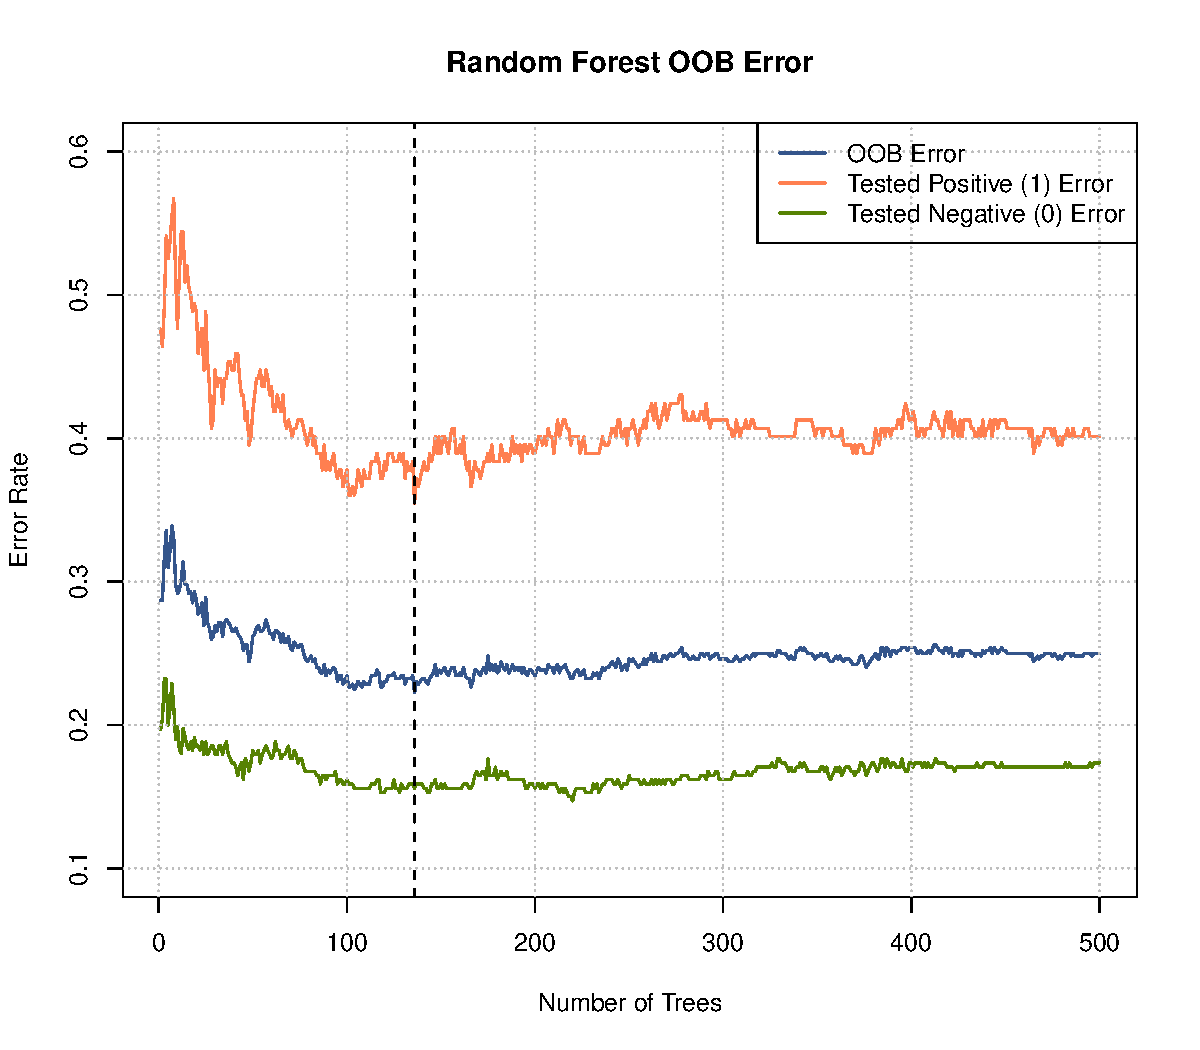
\includegraphics[width=1.05\columnwidth]{./Figures/forest/diabete_forest_error4.pdf}
\end{figure}
\end{column}
\end{columns}

\end{frame}

% ------------------------------- %

\begin{frame}%{Variable Importance}

\begin{figure}
\hspace*{-1.5em}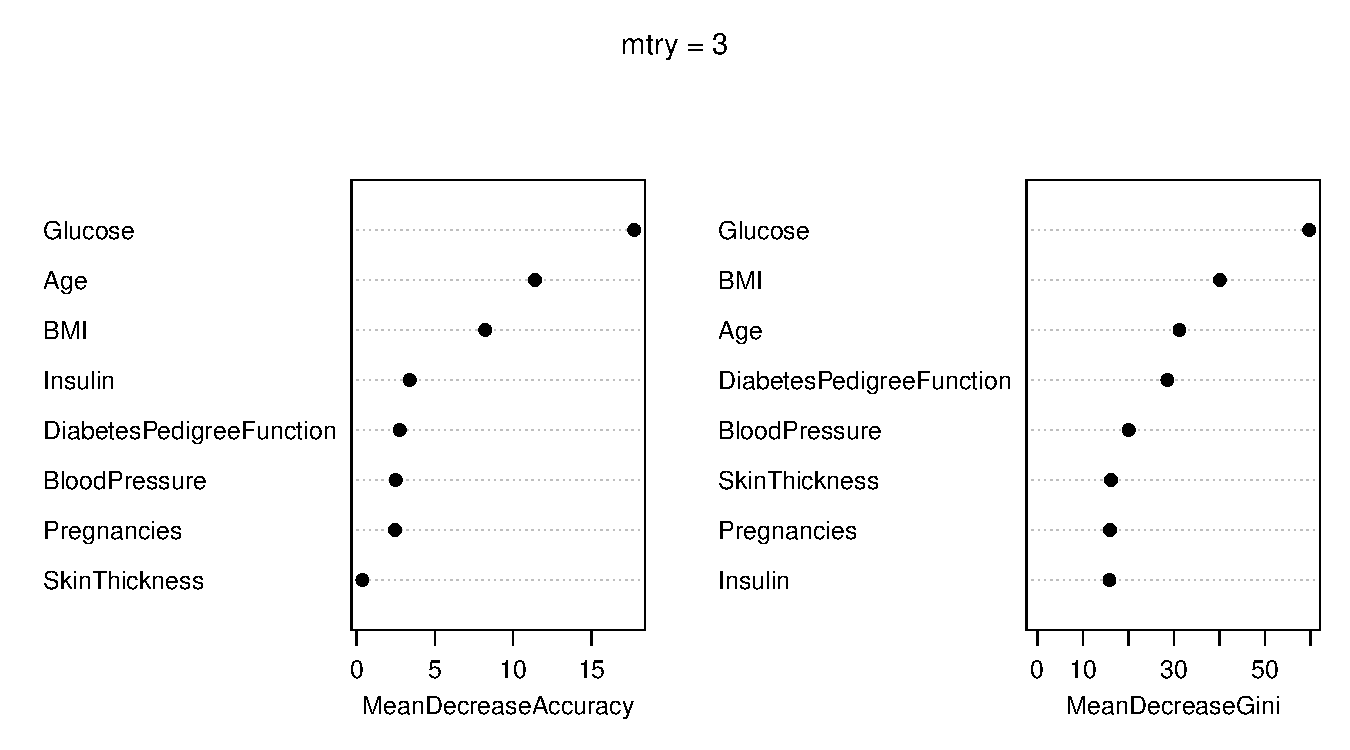
\includegraphics[width=0.78\textwidth]{./Figures/forest/diabete_var_imp3.pdf}
\hspace*{-1.5em}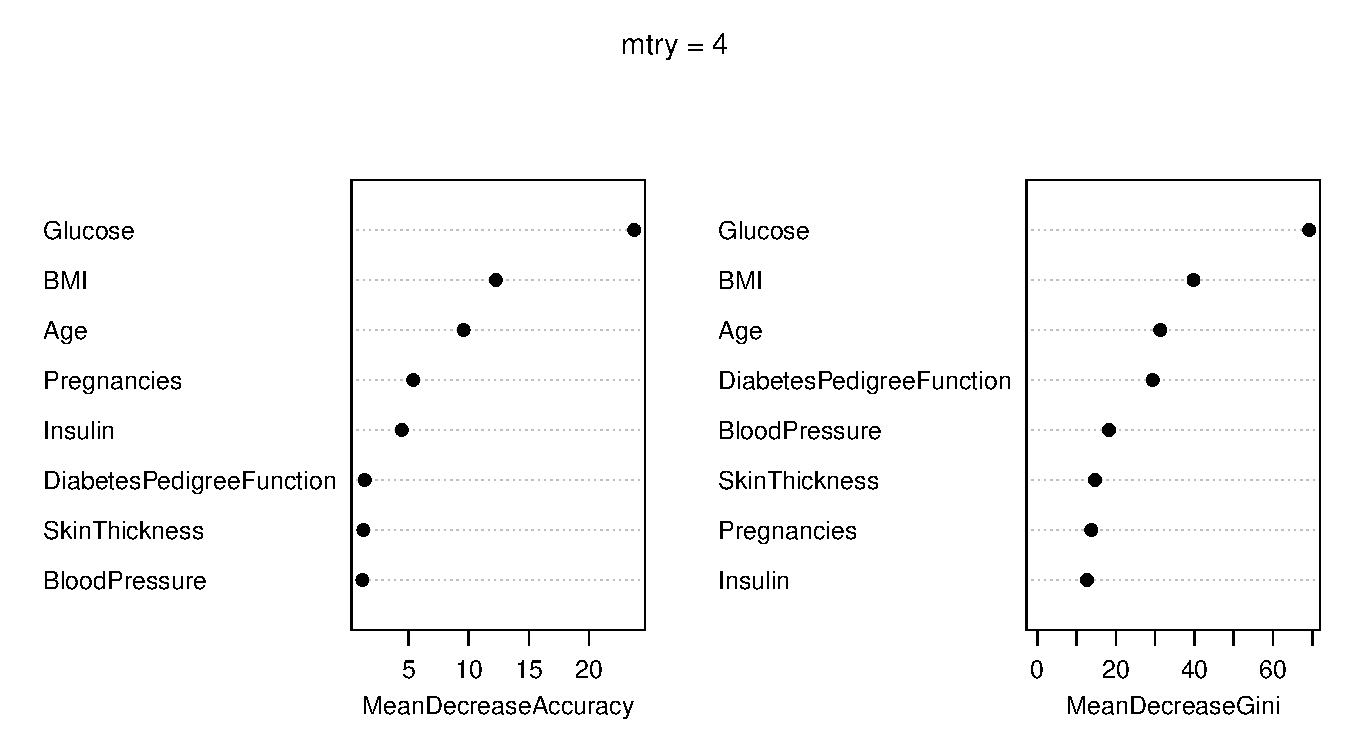
\includegraphics[width=0.78\textwidth]{./Figures/forest/diabete_var_imp4.pdf}
\end{figure}
\end{frame}

% ------------------------------- %

% !TeX spellcheck = en_GB

% ------------------------------- %
%% Introduction, AdaBoost classifier %%
% ------------------------------- %

\begin{frame}{The idea behind AdaBoost \,\,i}
What are we predicting?

$\mathcal{Y}\in\set{-1,1}$
\end{frame}

% ------------------------------- %

\begin{frame}{The idea behind AdaBoost \,\,ii}
%
\begin{columns}[T]
\begin{column}{0.48\textwidth}
\begin{figure}
\centering
\begin{tikzpicture}
	%draw,ellipse,fill=red!20,minimum height=2em,text centered,font=\sffamily\small
	\tikzset{help lines/.append style=pink}
	%\draw [help lines] (-2,-8) grid (3,1);

	\node[cloud] (m1) at (0,0) {training data};
	\node[cloud] (m2) at (0,-1.5) {weighted data};
	\node[cloud] (M) at (0,-4.5) {weighted data};
	\draw[-latex] (m1) to (m2);
	\draw[-,dotted,very thick] ($(m2.south) + (0,-0.15)$) to ($(M.north) + (0,+0.15)$);
	
	\node (G1) at (2.3,0) {$G_1(x)$};
	\node (G2) at (2.3,-1.5) {$G_2(x)$};
	\node (GM) at (2.3,-4.5) {$G_M(x)$};
	\draw[-stealth] (m1) to (G1);
	\draw[-stealth] (m2) to (G2);
%	\draw[-,dotted] (G2) to (GM);
	\draw[-stealth] (M) to (GM);
	
%	\node[rectangle,fill=pink!80] (G) at (1.5,-6) {$G(x)=\sign\Bigl(\sum_{m=1}^M\beta_mG_m(x)\Bigr)$};
	\node[rectangle,fill=mLightGreen!20] (G) at (1.5,-6.2) {$G(x)=\sign\Bigl(\sum_{m=1}^M\beta_mG_m(x)\Bigr)$};
%	\draw[-stealth] (GM) to (G);
\end{tikzpicture}
\end{figure}
\end{column}
\begin{column}{0.48\textwidth}
\vspace{0.7em}
Journey to the final classifier:
{\small\begin{itemize}
	\setlength{\itemsep}{-0.8ex}
	\item Linear combination of \alert{weak learners}
	\item Adaptively build up complexity
	\item Early stopping to achieve regularization
	\item \alert{Re-weighting} of training data  % permette all'algoritmo di concentrarsi sugli esempi più difficili da classificare, quindi di questi esempi viene aumentato il peso
\end{itemize}}
\vspace{1em}
Loss function:
$L(y,f(x))=\exp(-yf(x))$
%\begin{figure}
%\centering
%\begin{tikzpicture}
%	\begin{axis}[xlabel=$yf(x)$,ylabel={$L$},axis lines=middle,enlargelimits,width=0.9\textwidth]
%		\addplot[samples=200,blue,smooth] {exp(-x)};
%		%\addplot[dashed] {1};
%%		\addplot [black, mark=-, nodes near coords=$\log(2)$, font={\scriptsize}, every node near coord/.style={anchor=180}] coordinates {(0,{ln(2)})};
%	\end{axis}
%\end{tikzpicture}
%\end{figure}
\end{column}
\end{columns}

\end{frame}

% ------------------------------- %

\begin{frame}{Forward stagewise additive modeling}

The general framework for boosting  % additive expansion of basis functions

{%
\setlength{\interspacetitleruled}{0pt}%
\setlength{\algotitleheightrule}{0pt}%
\begin{algorithm}[H]
\KwIn{$M$, $\set{(x_i,y_i)}_1^N$}
Start with $f_0(\boldsymbol{x})=0$\;
\For{$m=1$ \KwTo $M$}{
%	Solve
	$(\beta_m,\gamma_m)=\argmin_{\beta,\gamma}\sum_{i=1}^NL(y_i,f_{m-1}(x_i)+\beta b(x_i;\gamma))$\;
%	Update
	$f_m(\boldsymbol{x})=f_{m-1}(\boldsymbol{x})+\beta_mb(\boldsymbol{x};\gamma_m)$\;
}
\end{algorithm}}

Where $b(\boldsymbol{x};\gamma_m)\in\R$ is a basis function depending on parameter $\gamma_m$ %  the number of basis functions is chosen according to hyper-parameter M
\end{frame}

% ------------------------------- %

\begin{frame}[fragile]{AdaBoost algorithm}

{%
\setlength{\interspacetitleruled}{0pt}%
\setlength{\algotitleheightrule}{0pt}%
\begin{algorithm}[H]
\KwIn{$M$, $\set{(x_i,y_i)}_1^N$}
Start with $f_0(\boldsymbol{x})=0$\;
\For{$m=1$ \KwTo $M$}{
	Compute weights $w_i^{(m)}=\exp(-y_if_{m-1}(x_i))$\;
	$G_m=\argmin_G\sum_{i=1}^Nw_i^{(m)}\mathbb{I}(y_i\neq G(x_i))$\;
%	$\text{err}_m$\;
	Compute $\beta_m=\frac{1}{2}\log\bigl(\frac{1-\text{err}_m}{\text{err}_m}\bigr)$\;
	Update $f_m(\boldsymbol{x})=f_{m-1}(\boldsymbol{x})+\beta_mG_m(\boldsymbol{x})$\;
}
\KwOut{$G(\boldsymbol{x})=\sign(f_M(\boldsymbol{x}))$}
\end{algorithm}}

Where the weak learner $G_m\in\set{-1,1}$ is a CART

\end{frame}

% ------------------------------- %

%%% metrics

% !TeX spellcheck = en_GB

% ------------------------------- %
%% Dataset, fitting, results %%
% ------------------------------- %

\begin{frame}{ModelX and cross-validation}
text\dots
\end{frame}

% ------------------------------- %

\begin{frame}{Metrics}

\begin{table}
\sisetup{round-mode=places}
\resizebox{0.65\textwidth}{!}{
\begin{tabular}{lS[round-precision=3]S[round-precision=3]}
	\toprule
	Model & {Metric1} & {Metric2} \\
	\midrule
	Model1 & 0.815971 & 0.667560 \\
	Model2 & 0.607353 & 0.666975 \\
	Model2 & 0.667406 & 0.464614 \\
	\bottomrule
\end{tabular}}
\end{table}

\end{frame}

% ------------------------------- %

%\appendix
%{\setbeamercolor{palette primary}{fg=black,bg=white}
%\begin{frame}[standout]
%%Thank you for your kindly attention!
%Questions?
%\end{frame}
%}

% ------------------------------- %


\appendix
\begin{frame}[allowframebreaks]{References}
\begin{thebibliography}{9}
	\bibitem{statslearn} T. Hastie, R. Tibshirani, and J. H. Friedman
	\newblock The Elements of Statistical Learning
	\newblock Springer, 6:191--199, 2009.
	% ---- %
	% add adaboost paper
	% add adaboost package
\end{thebibliography}
\end{frame}


\end{document}
